\appendixpage
\appendix
\chapter*{Appendices}
\addcontentsline{toc}{chapter}{List of Appendices}
\renewcommand{\thesection}{\Alph{section})}
\renewcommand{\thesubsection}{\Alph{section}.\arabic{subsection}}

\section{Queue Length Stabilisation}
\label{sec:Aqueuestabilization}
\subsection{Average Queue Length}
    \begin{figure}[h]
        \centering
        \begin{subfigure}[b]{0.475\textwidth}
            \centering
            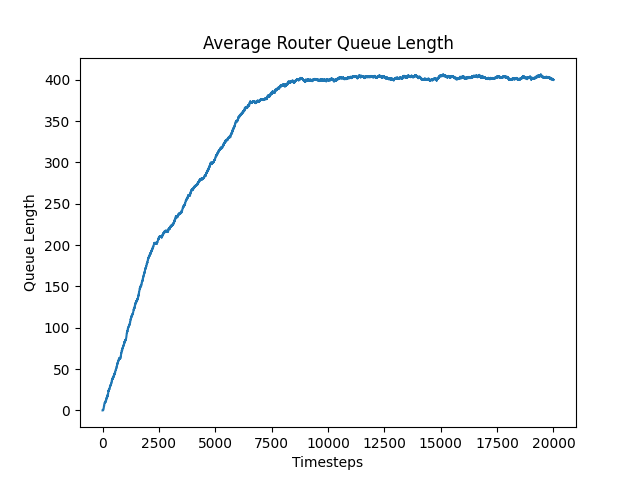
\includegraphics[width=\textwidth]{figs/appendix/average_ls=1.png}
            \caption[]{Average router queue length (LS update interval = 1)}
        \end{subfigure}
        \hfill
        \begin{subfigure}[b]{0.475\textwidth}
            \centering
            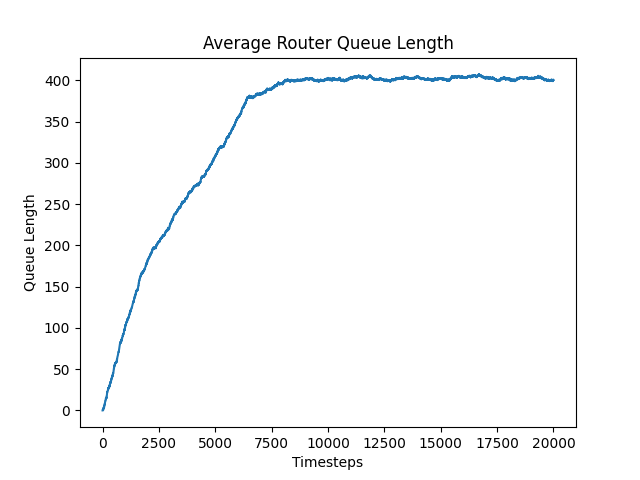
\includegraphics[width=\textwidth]{figs/appendix/average_ls=10.png}
            \caption[]{Average router queue length (LS update interval = 10)}
        \end{subfigure}
    \end{figure}
    \begin{figure}[H]\ContinuedFloat
        \centering
        \begin{subfigure}[b]{0.475\textwidth}
            \centering
            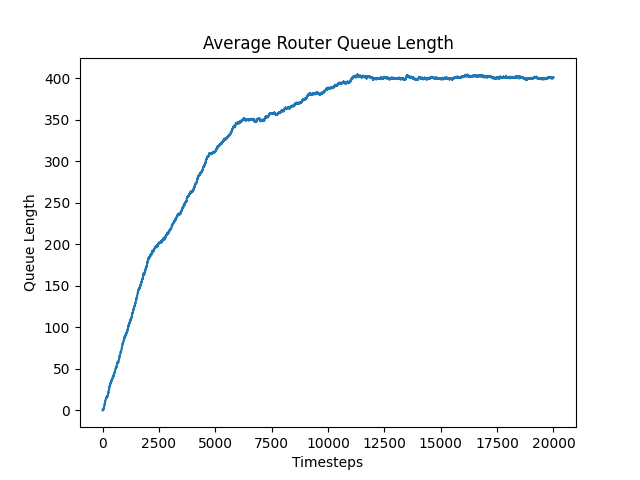
\includegraphics[width=\textwidth]{figs/appendix/average_ls=50.png}
            \caption[]{Average router queue length (LS update interval = 250)}
        \end{subfigure}
        \hfill
        \begin{subfigure}[b]{0.475\textwidth}
            \centering
            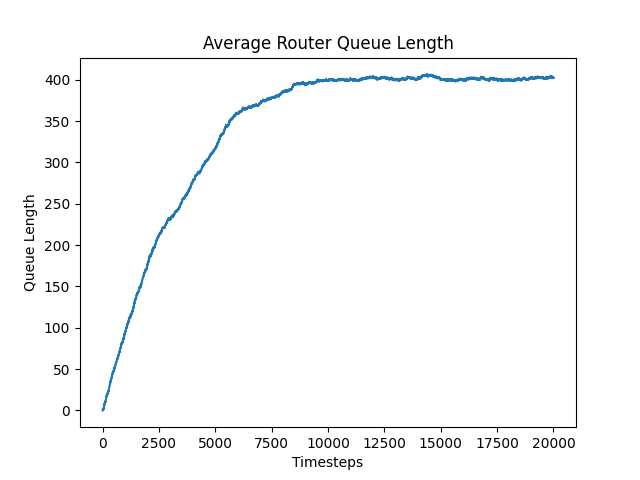
\includegraphics[width=\textwidth]{figs/appendix/average_ls=500.png}
            \caption[]{Average router queue length (LS update interval = 500)}
        \end{subfigure}
    \end{figure}
    \begin{figure}[H]\ContinuedFloat
        \centering
        \begin{subfigure}[t]{0.475\textwidth}
            \centering
            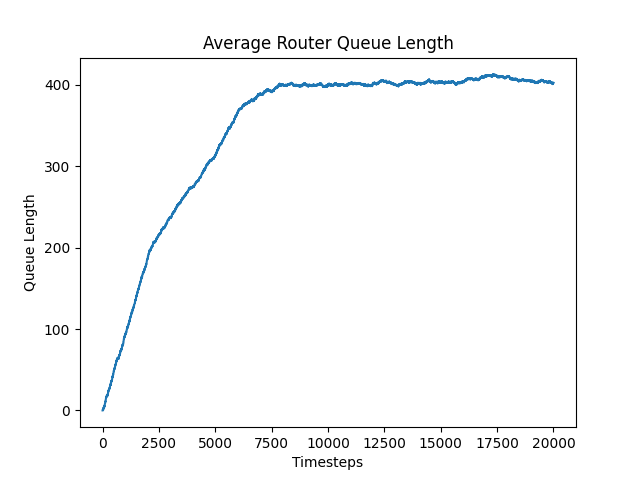
\includegraphics[width=\textwidth]{figs/appendix/average_ls=1000.png}
            \caption[]{Average router queue length (LS update interval = 1000)}
            \label{fig:avgq-1000}
        \end{subfigure}
        \hfill
        \begin{subfigure}[t]{0.475\textwidth}
            \centering
            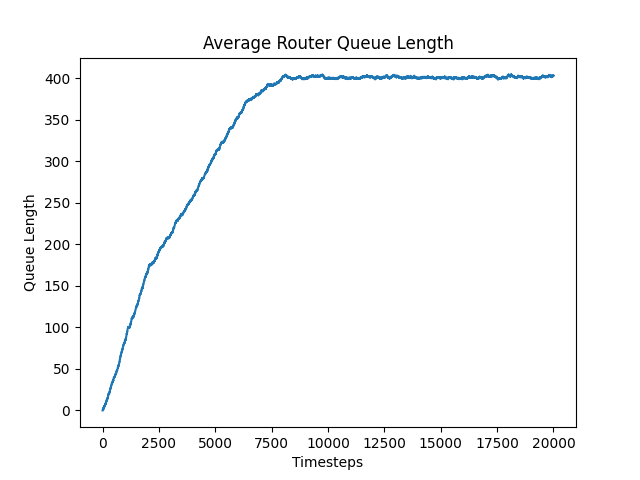
\includegraphics[width=\textwidth]{figs/appendix/average_ls=10000.png}
            \caption[]{Average router queue length (LS update interval = 10000)}
            \label{fig:avgq-10000}
        \end{subfigure}
    \end{figure}
    
\subsection{Variance of Queue Length}
\lfix{Trim variance graphs to same length as averages}
    \begin{figure}[H]
        \centering
        \begin{subfigure}[b]{0.475\textwidth}
            \centering
            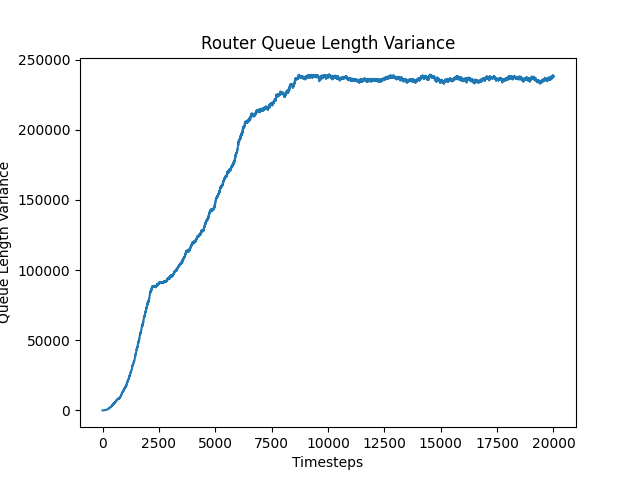
\includegraphics[width=\textwidth]{figs/appendix/variance_ls=1.png}
            \caption[]{Variance of router queue length (LS update interval = 1)}
            \label{fig:qvar-1}
        \end{subfigure}
        \hfill
        \begin{subfigure}[b]{0.475\textwidth}
            \centering
            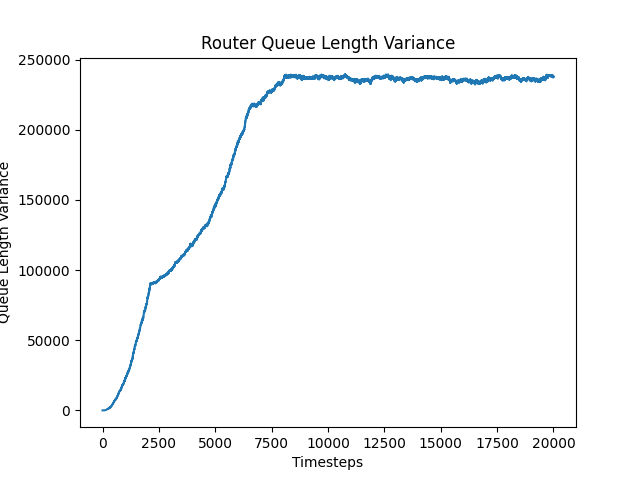
\includegraphics[width=\textwidth]{figs/appendix/variance_ls=10.png}
            \caption[]{Variance of router queue length (LS update interval = 10)}
            \label{fig:qvar-10}
        \end{subfigure}
    \end{figure}
    \begin{figure}[H]\ContinuedFloat
        \centering
        \begin{subfigure}[b]{0.475\textwidth}
            \centering
            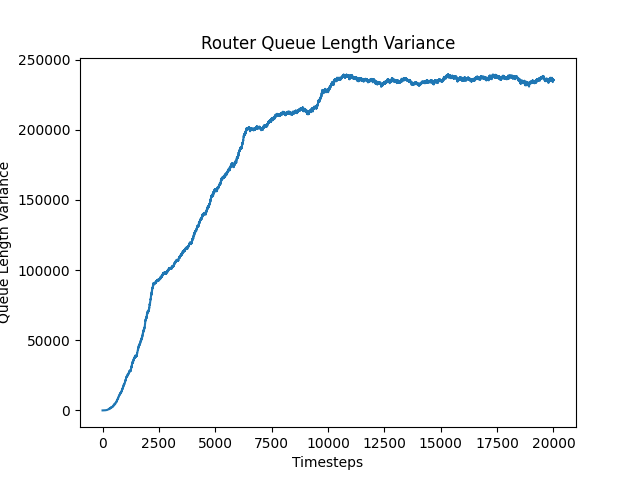
\includegraphics[width=\textwidth]{figs/appendix/variance_ls=250.png}
            \caption[]{Variance of router queue length (LS update interval = 250)}
            \label{fig:qvar-250}
        \end{subfigure}
        \hfill
        \begin{subfigure}[b]{0.475\textwidth}
            \centering
            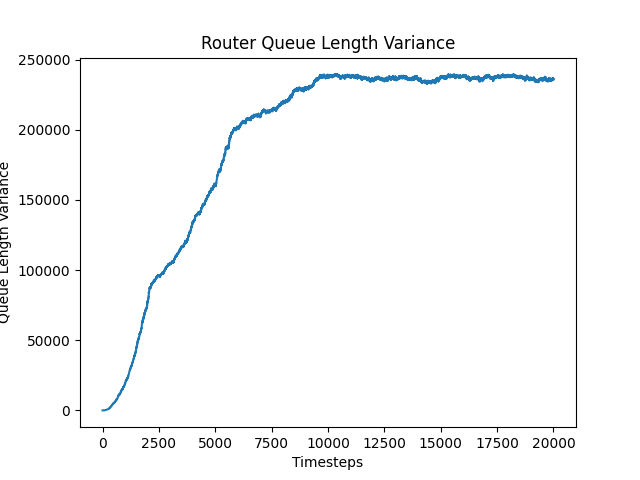
\includegraphics[width=\textwidth]{figs/appendix/variance_ls=500.png}
            \caption[]{Variance of router queue length (LS update interval = 500)}
            \label{fig:qvar-500}
        \end{subfigure}
    \end{figure}
    \begin{figure}[H]\ContinuedFloat
        \begin{subfigure}{0.475\textwidth}
            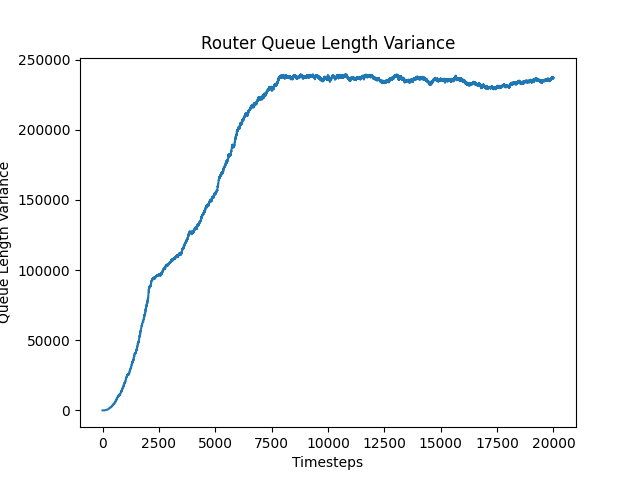
\includegraphics[width=\textwidth]{figs/appendix/variance_ls=1000.png}
            \caption[]{Variance of router queue length (LS update interval = 1000)}
            \label{fig:qvar-1000}
        \end{subfigure}
        \hfill
        \begin{subfigure}[H]{0.475\textwidth}
            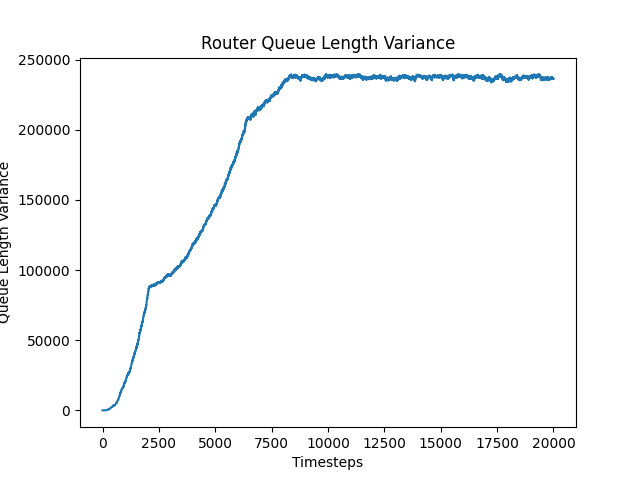
\includegraphics[width=\textwidth]{figs/appendix/variance_ls=10000.png}
            \caption[]{Variance of router queue length (LS update interval = 10000)}
            \label{fig:qvar-10000}
        \end{subfigure}
    \end{figure}

\captionsetup{justification=centering}
\begin{figure}[H]
    \centering
    \begin{subfigure}{0.475\textwidth}
        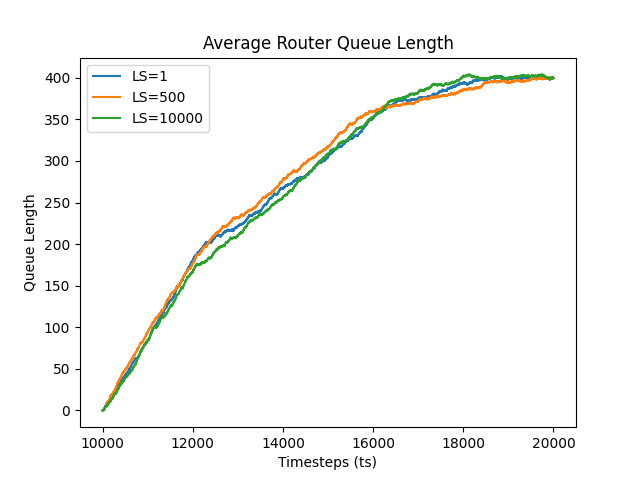
\includegraphics[width=\textwidth]{figs/appendix/average_of_1,500,10000.png}
        \caption{Average.}
        \label{fig:Ravgq}
    \end{subfigure}
    \hfill
    \begin{subfigure}{0.475\textwidth}
        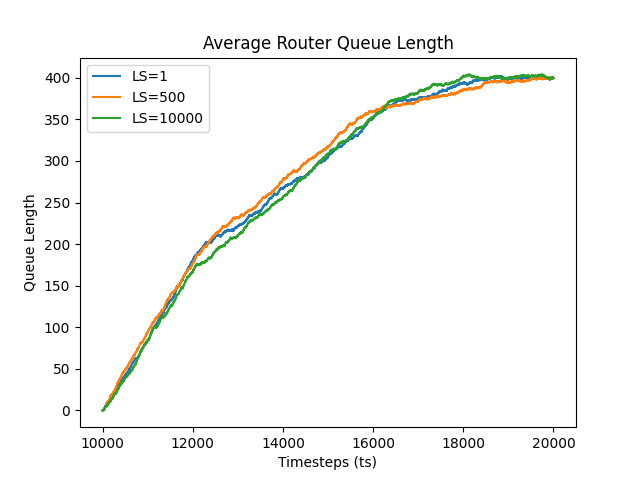
\includegraphics[width=\textwidth]{figs/appendix/average_of_1,500,10000.png}
        \caption[]{Variance.}
        \label{fig:Rvarq}
    \end{subfigure}
    \caption{Mean and variance of router queue buffer lengths over link-state update intervals 1, 500, and 10,000].}
\end{figure}

\begin{table}[H]
    \centering\sisetup{table-number-alignment=center}
    \begin{tabular}{@{}lS[table-format=1.2e1]c@{}}
        \toprule
        \multirow{2}{*}{\makecell{LS Update \\ Interval}} & \multicolumn{2}{@{}S@{}}{\textbf{Time-step range}}\\
        \cmidrule(rl){2-3}
        & {$\leq$ 20,000} & {> 20,000} \\
        \midrule
        1       & 1.07E4 & 6.25 \\ 
        10      & 1.02e4 & 4.88 \\
        50      & 1.01e4 & 3.21 \\
        250     & 1.07e4 & 5.06 \\
        500     & 1.01e4 & 6.05 \\
        1,000   & 1.03e4 & 3.47 \\
        10,000  & 1.12e4 & 5.22 \\
        \bottomrule
    \end{tabular}
    \caption{Variance pre and post queue length stabilization point}
\end{table}

\newpage

\newpage
\section{Mapping of Packet Delay Metrics to Hold Probability}
\label{sec:APDAtoHoldprob}
 To establish a relationship between router packet delay metrics and hold probability we  consider 100 randomly generated topologies between 10-50 nodes, 50 generated using BA and 50 using ER. Randomly generated topologies are used in-place of the limited number real world topologies to ensure results are robust. We assume that there is an underlying parameterised relationship between a routers hold probability and buffer queue length. With the relationship being parameterised over the two variable network parameters: max buffer queue length and background traffic intensity.\par
  To determine this relationship we simulate each topology with a combinations of max queue length from  200-5,000 and background traffic intensity from 0.1-0.5, each for 10,000 time steps. For each combination of parameters the hold probability of a randomly selected nefarious router is varied from 0.1-0.9. The PDA of the router is recorded along with the corresponding hold probability. Results are then graphed using a scatter plot to visually approximate and display the relationship between these router attributes. For implementation details see \cite{sylvester_millar_real_2021}.\par
  To map an arbitrary hold value to a measured PDA or vice-versa we fit a function to these discrete observed data points. The data is fitted using the curve\_fit function of SciPy's optimize class which we provide an initial guess of parameters. We tested multiple possible function to fit the data but a standard sigmoid function was found to fit best, matching initial visual analysis of the distribution. We provided the curve function with a minimum value of 0 and a maximum of the maximum queue length. The Levenberg–Marquardt minimisation algorithm was used for fitting as it was found to be the best performing of algorithms within SciPy's library. For transparency we also present results for curve fitting using Trust Region Reflective and Rectangular Trust Region Dogleg minimisation algorithms.\par
  We record the estimated curve fitting parameters from SciPy's curve fitting, noting the minimum and maximum values are approximately the supplied initial guesses. Finally, variation of the functions parameters w.r.t max queue length and background traffic intensity were modeled. This enabled estimation of the PDA to hold probability relation given only network parameters.\par
  Inverting the observed empirical PDA from varying hold probabilities we are able to estimate hold probability from PDA alone. Using this estimation of hold probability we select a hold probability between 0.0-1.0 as a threshold for a router being classified as nefarious. We then generate a ROC curve to evaluate the efficacy of our classification in the most general context possible. We do not present a confusion matrix  as requirements governing tolerated number of false negatives and false positive will vary between systems.\par
  
  We consider the baseline network in \cref{fig:A6routertop} for initial analysis we pivot to examination of the validity of our new inferential method under varied network conditions. The two primary dynamic properties in the simulated network are the length of router queuing buffers and the amount of background traffic which we refer to as traffic intensity. We consider the impact of these properties and their combinatory effects on packet delay metrics.\par
  \begin{figure}[H]
    \centering
    \tikzsetnextfilename{6routertopology_appendix}
    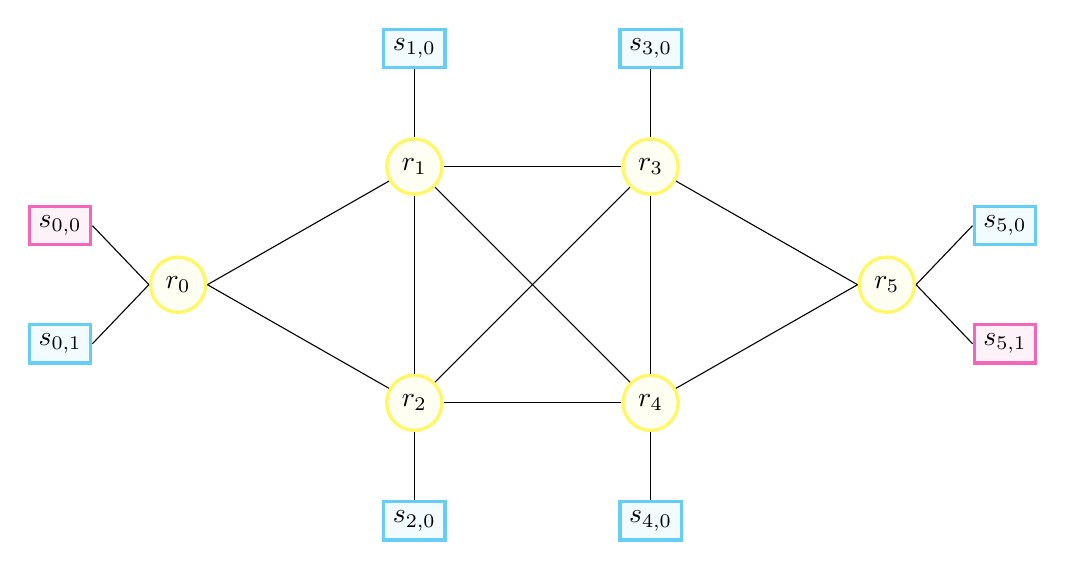
\begin{tikzpicture}[
        router/.style={circle, draw=yellow!60, fill=yellow!5, very thick, minimum size=3.5mm},
        nef_router/.style={circle, draw=red!60, fill=red!5, very thick, minimum size=3.5mm},
        switch/.style={rectangle, draw=cyan!60, fill=cyan!5, very thick, minimum size=2.5mm},
        monitor/.style={rectangle, draw=magenta!60, fill=magenta!5, very thick, minimum size=2.5mm},]
        
        % Routers
        \node[router] (r0) at (-4.5,0)    {$r_0$};
        \node[router] (r1) at (-1.5,1.5)  {$r_1$};
        \node[router] (r2) at (-1.5,-1.5) {$r_2$};
        \node[router] (r3) at (1.5,1.5)   {$r_3$};
        \node[router] (r4) at (1.5,-1.5)  {$r_4$};
        \node[router] (r5) at (4.5,0)     {$r_5$};
        
        %Switches
        \node[monitor](s00) at (-6,.75)   {$s_{0,0}$};
        \node[switch] (s01) at (-6,-.75)  {$s_{0,1}$};
        \node[switch] (s10) at (-1.5,3)   {$s_{1,0}$};
        \node[switch] (s20) at (-1.5,-3)  {$s_{2,0}$};
        \node[switch] (s30) at (1.5,3)   {$s_{3,0}$};
        \node[switch] (s40) at (1.5,-3)   {$s_{4,0}$};
        \node[switch] (s50) at (6,.75)   {$s_{5,0}$};
        \node[monitor](s51) at (6,-.75)   {$s_{5,1}$};
        %Links
        \draw[-] (r0.east) -- (r1);
        \draw[-] (r0.east) -- (r2);
        \draw[-] (r1) -- (r2);
        \draw[-] (r1) -- (r3);
        \draw[-] (r1.south east) -- (r4.north west);
        \draw[-] (r2) -- (r3);
        \draw[-] (r2) -- (r4);
        \draw[-] (r3) -- (r4);
        \draw[-] (r3) -- (r5.west);
        \draw[-] (r4) -- (r5.west);
        \draw[-] (s00.east) -- (r0.west);
        \draw[-] (s01.east) -- (r0.west);
        \draw[-] (s10) -- (r1);
        \draw[-] (s20) -- (r2);
        \draw[-] (s30) -- (r3);
        \draw[-] (s40) -- (r4);
        \draw[-] (s50.west) -- (r5.east);
        \draw[-] (s51.west) -- (r5.east);
    \end{tikzpicture}
    \caption{6 router network with 2 monitors located at $r_0$ and $r_5$ (Reprinted from page \pageref{fig:6routersample})}
    \label{fig:A6routertop}
\end{figure}\par
We consider only the case of $r_1$ begin nefarious, we measure the impact of hold probabilities on packet delay metrics over varying buffer queue lengths. Firstly considering PDA plots of original values and values with a standard min-max normalisation applied are given in \cref{fig:Rvariedqlenpda}.\par
From these we see that irrespective of queue length the relation between hold probability and PDA appears to be a sigmoid curve. Using a standard Levenberg–Marquardt method \cite{osborne_nonlinear_1976} we fit a sigmoid curve of the form $x=a/1+e^{-c\cdot x-d} + b$ to each set of observation results. We selected the Levenberg–Marquardt minimisation algorithm as it performed the best over all fits, both the trust region reflective algorithm and dogleg algorithm with a rectangular trust region were tried but produced inferior $R^2$ values, results for these fits are shown in \cref{Aaltcurvefit}.\par
The fit was calculated to have an $R^2=0.997$ with a minimum of $R^2=0.994$, accurate enough to confirm the initial prediction. In the non-normalised case the upper bound of each sigmoid is given by approximately the maximum length and a lower bound being approximately 0. In normalising the data we see that an increase in queue length both shifts the inflection point of the sigmoid to the right and reduces the gradient of the inflection. The exception to this is queue lengths < 50 where the function seems to behave strangely, we anticipate this is due to the queue easily becoming full, thereafter dropping packets and containing less information, queue lengths this small would however be in practical in real world systems, as such we do not consider these in further analysis and leave them to future work.\par
\begin{figure}[H]
    \centering
    \begin{subfigure}{0.475\textwidth}
        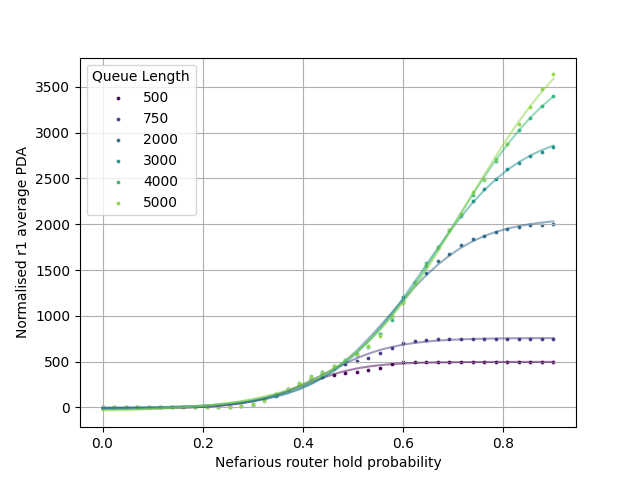
\includegraphics[width=\textwidth]{figs/results/qlen_fitting/qlen_PDA_lm.png}
        \caption{Original}
    \end{subfigure}
    \begin{subfigure}{0.475\textwidth}
        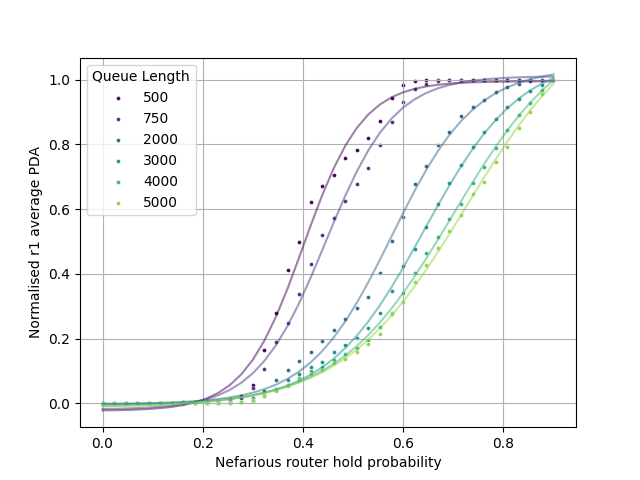
\includegraphics[width=\textwidth]{figs/results/qlen_fitting/norm_qlen_PDA_lm.png}
        \caption{Min-max scaled}
    \end{subfigure}
    \caption{Plots of average nefarious router buffer queue length over various hold probabilities.}
    \label{fig:Rvariedqlenpda}
\end{figure}
  
  \label{Aaltcurvefit}
\begin{figure}[H]
    \centering
    \begin{subfigure}{0.475\textwidth}
        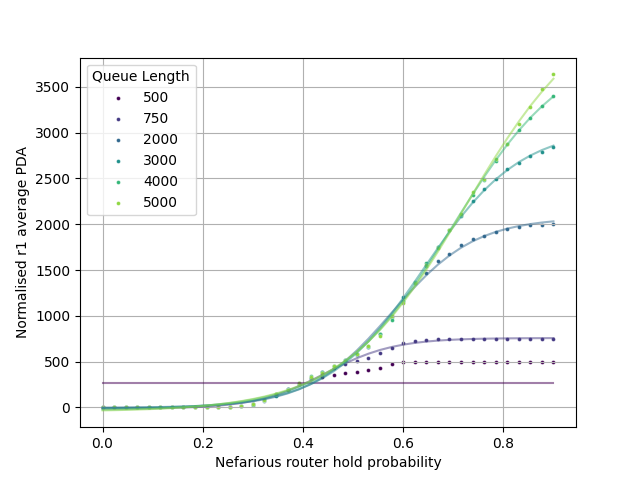
\includegraphics[width=\textwidth]{figs/results/qlen_fitting/qlen_PDA_trf.png}
        \caption{Original}
    \end{subfigure}
    \begin{subfigure}{0.475\textwidth}
        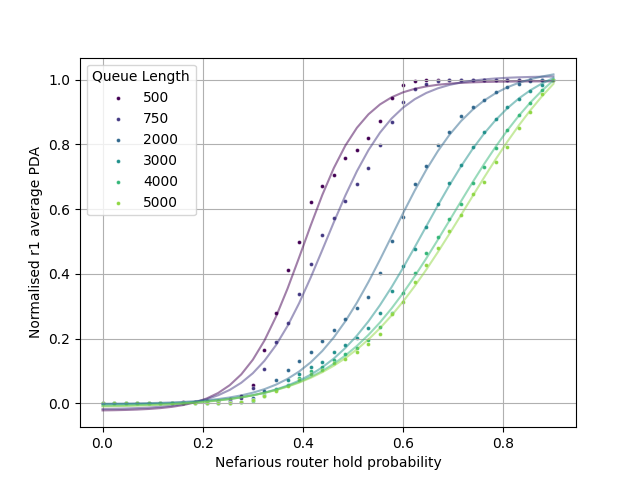
\includegraphics[width=\textwidth]{figs/results/qlen_fitting/norm_qlen_PDA_trf.png}
        \caption{Min-max scaled}
    \end{subfigure}
    \caption{Plots of average nefarious router buffer queue length over various hold probabilities fitted using TRF minimisation.}
\end{figure}

\begin{figure}[H]
    \centering
    \begin{subfigure}{0.475\textwidth}
        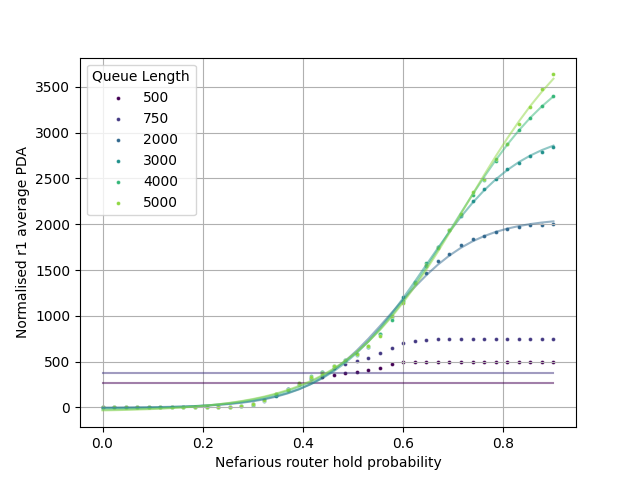
\includegraphics[width=\textwidth]{figs/results/qlen_fitting/qlen_PDA_dogbox.png}
        \caption{Original}
    \end{subfigure}
    \begin{subfigure}{0.475\textwidth}
        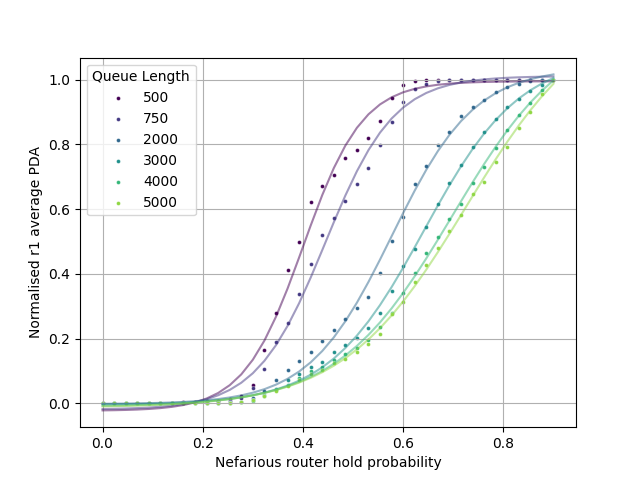
\includegraphics[width=\textwidth]{figs/results/qlen_fitting/norm_qlen_PDA_dogbox.png}
        \caption{Min-max scaled}
    \end{subfigure}
    \caption{Plots of average nefarious router buffer queue length over various hold probabilities fitted using dogbox minimisation.}
\end{figure}

\begin{table}[H]
 \centering
  \begin{tabular}{@{}cccccc@{}}
   \toprule
    &&\multicolumn{2}{c}{\textbf{PDA}} & \multicolumn{2}{c}{\textbf{PDV}} \\
    \cmidrule(rl){3-4} \cmidrule(rl){5-6}
    Algorithm & $R^2$ & Original & Scaled & Original & Scaled \\
    \midrule
    \multirow{2}{*}{LM}     & $\overline{x}$ & 99.778        & 99.778 & 99.187 & 99.187 \\
                            & min            & 99.403        & 99.403 & 98.323 & 98.323 \\
    \multirow{2}{*}{TRF}    & $\overline{x}$ & 83.211        & 99.778 & -      & 99.187 \\
                            & min            & 5.679         & 99.403 & -      & 98.323 \\
    \multirow{2}{*}{Dogbox} & $\overline{x}$ & 66.595        & 99.778 & -      & 99.187 \\
                            & min            & 6.399$e^{-9}$ & 99.403 & -      & 98.323 \\
   \bottomrule
  \end{tabular}
  \caption{Variance of nefarious router PDA grouped by varying delay probabilities in the baseline 6 router network. (Note all values are $R^2\cdot 100$)}
  \end{table}
    
    To quantify the relationship between queue length and the produced sigmoid we calculate the coefficients for the point of inflection and gradient for each queue length in \cref{fig:Rsigmoidcoefs}. A clear decreasing logarithmic trend can be seen between queue length and inflection point, with an increasing polynomial trend between queue length and inflection gradient. Fitting a polynomial model to this trend we are able to produce a function to estimate the sigmoid curve given a routers queue length. This estimation can allow for the relation to be inverted i.e. given a router's queue length and PDA we can estimate the router's hold probability.
    \begin{figure}[H]
        \centering
        \begin{subfigure}{0.475\textwidth}
            
\includegraphics[width=\textwidth]{figs/results/qlen_param_c.png}
            \caption{Gradient at inflection point}
        \end{subfigure}
        \begin{subfigure}{0.475\textwidth}
            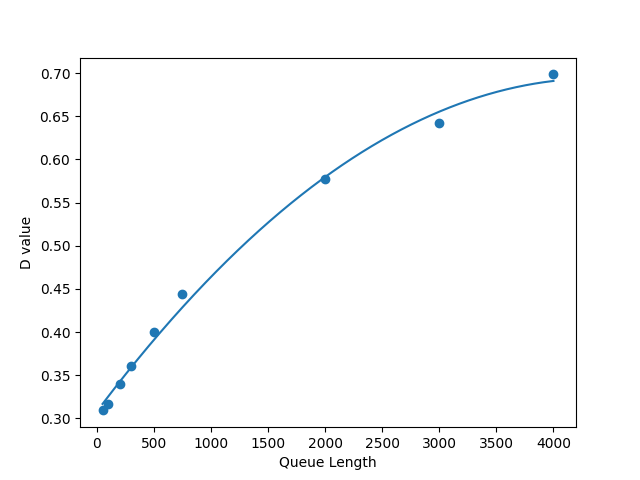
\includegraphics[width=\textwidth]{figs/results/qlen_param_d.png}
            \caption{X-value of infection point}
        \end{subfigure}
        \caption{Plots of parameters for modeled sigmoid relationship between hold probability and router buffer queue length.}
        \label{fig:Rsigmoidcoefs}
    \end{figure}